\chapter{Webový server}
Webový server je~nejdůležitější a~nejobsáhlejší část celého systému. 
Webový server mám nasazený na mikropočítači~Raspberry Pi 4 Modelu B který má 8~GB operační paměti.
Toto zařízení jsem zvolil hlavně kvůli nízké spotřebě elektrické energie a~velké komunitě lidí, kteří tento mikropočítač využívají.

Na zařízení běží operační systém Raspberry Pi OS s~grafickým rozhraním.
Webové stránky běží na HTTP serveru Apache2 a~PHP 7.3.
Jako databázový systém využívám MariaDB.
Server běží lokálně uvnitř firmy na zabezpečené sítí, tím pádem není nutné velké zabezpečení systému.
\fxnote[author=JA]{\textcolor{mygreen}{Zabezpečení přepsat jinak}}
Z~toho také vyplývá, že stránka je dostupná pouze ve vnitřní síti firmy.  
Celý webový server mám verzovaný také na GitHubu.\newline
GitHub: \href{https://github.com/Pletacka-IoT/Pletacka-website}{Pletacka-website}\cite{PL_WEB}

%SECTION
\section{Frontend}
% Frontend neboli vizuální část webové stránky je pro uživatele ta nejdůležitější.
% Webový design musí zaujmout a~udržet si diváka.
% V~aktuální době plné mobilních telefonů je důležité aby se aplikace správně zobrazovala i~na takto malých zařízeních.
 
Frontend je vizuální část webové stránky zobrazená uživatelem.
Pomocí frontendu se na obrazovku vykresluje veškerý text a~jednotlivé prvky stránky.

\subsection{Bootstrap}
Bootstrap je knihovna sloužící k~jednoduchému a~rychlému vytvoření responzivních webových stránek.
Díky této knihovně jsou stránky správně zobrazovány i~na mobilních zařízeních.
Tento nástroj se vyvíjí od roku 2011 a~je pod otevřenou licencí.
Webový server využívá Bootstrap verze čtyři.


\subsection{JavaScript}
Na frontendu používám JavaScript společně s~technologií AJAX pro aktualizaci částí stránek. AJAX umožňuje překreslovat jen určitou část obsahu stránky bez nutnosti načíst celou stránku znovu.
Tím se zásadně zrychluje načítání a~interaktivita stránek. Dochází i~k~značné úspoře přenesených dat.
K~tomuto efektivnímu překreslování slouží knihovna Naja\cite{NAJA}, kterou napsal český vývojář Jiří Pudil.
Knihovna také nabízí jednoduchou integraci do PHP frameworku Nette, o~kterém budu psát dále.   



%SECTION
\section{Backend}
Je to nejobsáhlejší část celé této práce. 
Backend je serverová část webových stránek, neběží tedy u~vás~na počítači~jako frontend, ale na webovém serveru.   
Celý backend systému Pletačka IoT jsem napsal v~programovacím jazyce PHP a~ve frameworku Nette\cite{NETTE}, který nabízí ucelenou sadu nástrojů k~tvorbě webu.
Backend se stará o~přijímání dotazů ze senzorů a~následný zápis do databáze, pohání celý webový server a~vytváří databázové výběry.
Nejdříve zde popíšu~použité technologie a~následně rozeberu jednotlivé stránky aplikace.

\subsection{PHP}
Webovou aplikaci programuji v~PHP ve verzi 7.3. Jako programovací studio jsem zvolil studentskou verzi aplikace PHPStorm, která je velmi mocným nástrojem při~tvorbě webu.
Testovací verze aplikace mám spuštěnou na svém počítači~kde také celý tento systém vyvíjím. 

Pro snadnější ladění chyb používám Xdebug, díky kterému si můžu~krokovat jednotlivé řádky kódu a~rychleji tak nalézt chybu.

Jako systém pro správu balíčků používám nástroj Composer, který se ovládá z~terminálu pomocí jednoduchých příkazů.
Umožňuje rychlou definici závislostí a~aktualizaci všech modulů pomocí jednoho příkazu.


\subsection{Nette}
Nette je webový framework vyvíjený komunitou. Vznikl v~České republice a~jeho zakladatelem je David Grudl. 
Nabízí vlastní šablonovací jazyk, na jednoduché a~efektivní vykreslování webových stránek. 
Nette disponuje obsáhlou a~velmi dobře zpracovanou dokumentací, ale také velkou komunitou lidí kteří s~tímto frameworkem pracují a~velmi dobře mu rozumí. 


\subsection{Web API}

\fxnote[author=JPA]{\textcolor{mygreen}{Chtěl bych se ještě pobavit o~definici/popisu Web API}}

Web API je soubor příkazů ke komunikaci s~webovou stránkou.
Webová stránka Pletačka IoT obsahuje základní sadu web API.
Primárně ji využívají senzory k~odesílání naměřených dat a~ke zpětnému posílání odpovědí do senzoru.
Druhé využití API je k~vytváření databázových výběrů, to je voláno nástrojem na automatizaci procesů v~nastavený čas. 


%SECTION
\section{Webové rozhraní Pletačka IoT}
Každá stránka stránka je rozdělena na tři~části. Záhlaví, to obsahuje logo a~odkazy na nejpoužívanější stránky.
Druhou částí jsou samotné webové stránky které budou popsány v~dalších odstavcích.
Poslední částí je minimalistické zápatí s~copyright znakem.\newline
Stránky Pletačky jsem navrhoval tak, aby splňovaly tyto parametry:

\fxnote[author=JA]{\textcolor{mygreen}{Doplnit obrázky stránek pod kapitolu nebo jeden list s~fotkami}}

\begin{itemize}
    \item jednoduché rozhraní pro uživatele
    \item přehledné zobrazení dat
    \item zobrazovat pouze užitečná dat
    \item rychlá editace senzorů
    \item využití číselných identifikátorů
\end{itemize}


\subsection{Úvodní stránka}
V~horní části úvodní stránky se vypisují tři~nejpodstatnější údaje.
Jde o~celkový počet upletených párů za aktuální směnu.
Dále pak úspěšnost vypočítávanou z~času zastavení stroje a~z~celkové času zapnutí stroje.
Posledním údajem je průměrná doba stání jednoho stroje.   

Pod těmito čísly se zobrazuje tabulka s~barevnými obdélníky, kde každý představuje jeden stroj.
Barva obdélníků udává aktuální stav stroje a~text v~pozadí tuto informaci doplňuje. 

\begin{figure}[htbp]
    \centering
    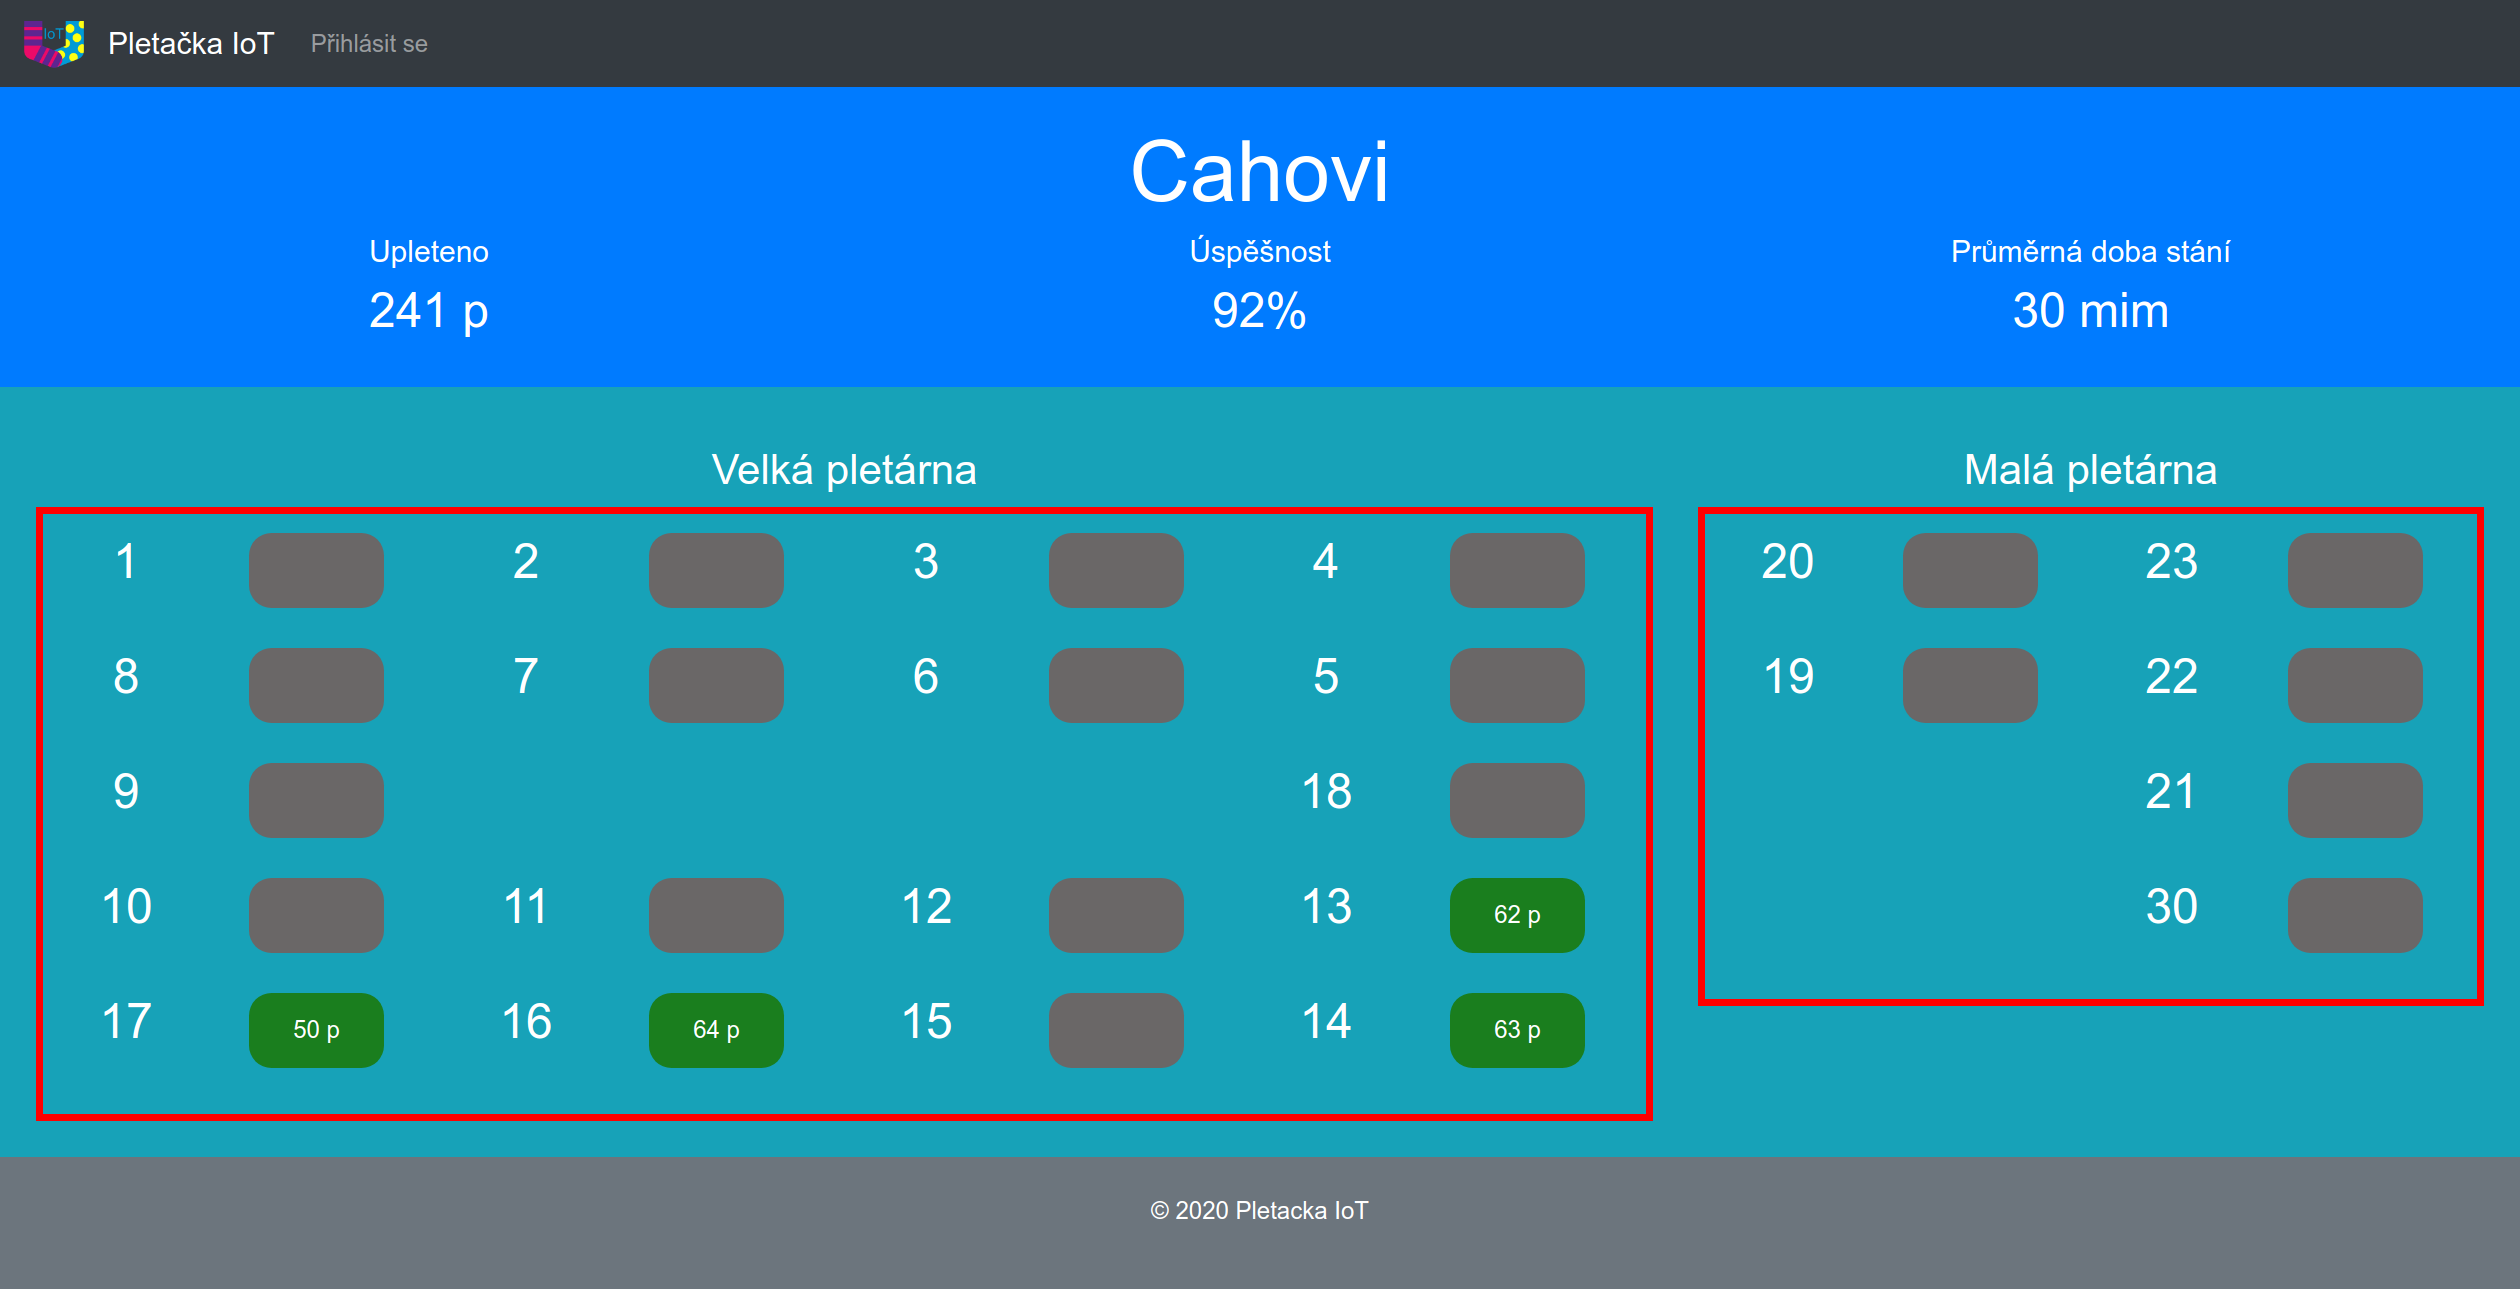
\includegraphics[width=\textwidth]{img/Home.png}
    \caption{Úvodní stránka}
    \label{fig:webUvod}
\end{figure}

%\subsection{Přehled ze senzoru} 
Po kliknutí na senzor na úvodní stránce, se zobrazí data o~právě vybraném stroji.
Veškerá data jsou rozdělena do dvou sloupců podle pracovních směn.
To umožňuje zaměstnavateli jednoduché porovnávání pracovních směn.
V~úvodu každého sloupce je obecný přehled naměřených dat za různá období.
Pod nimi je přehled v~grafech a~porovnání nejdůležitější údajů.

\begin{figure}[htbp]
    \centering
    % 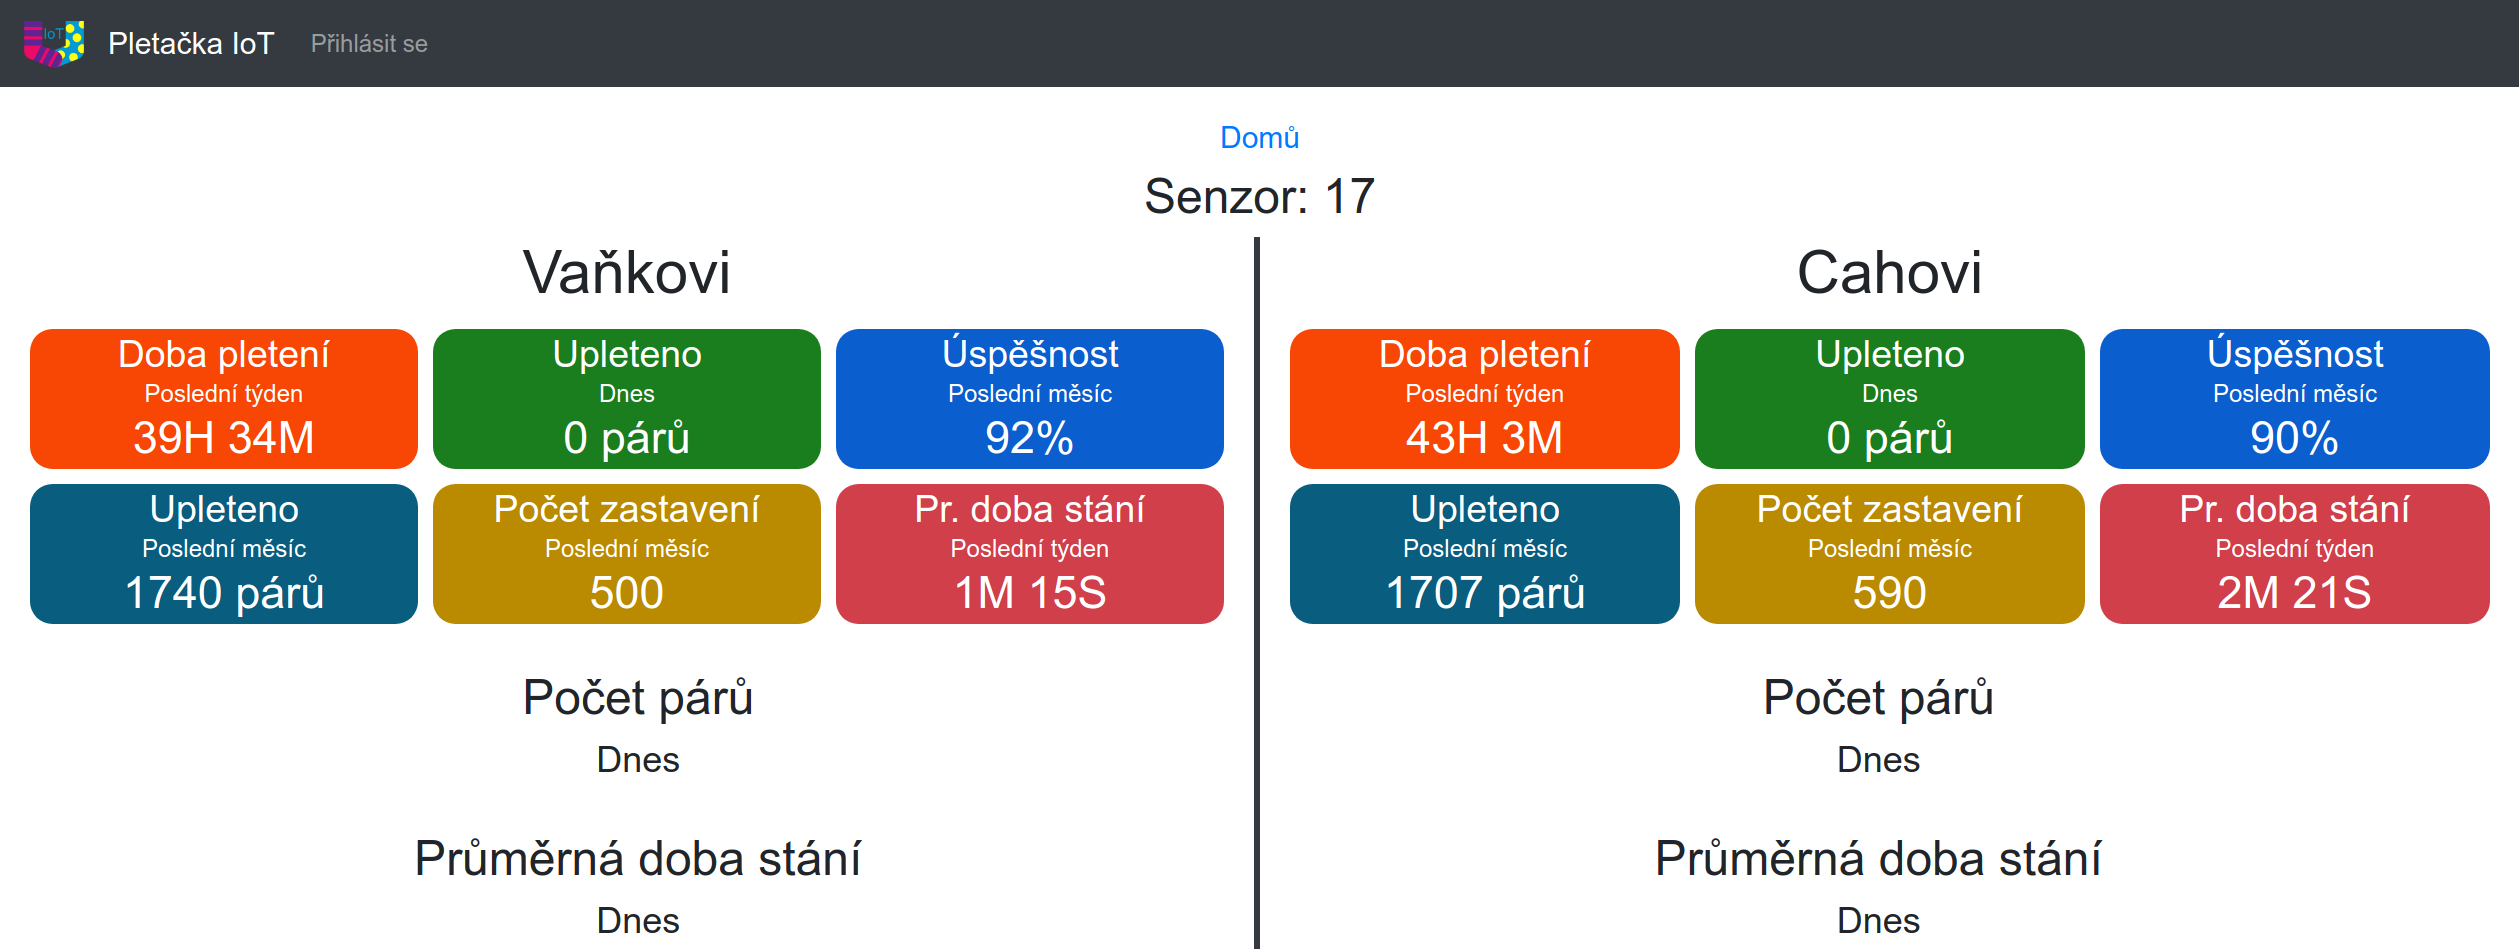
\includegraphics[width=\textwidth]{img/Senzor.png}
    % 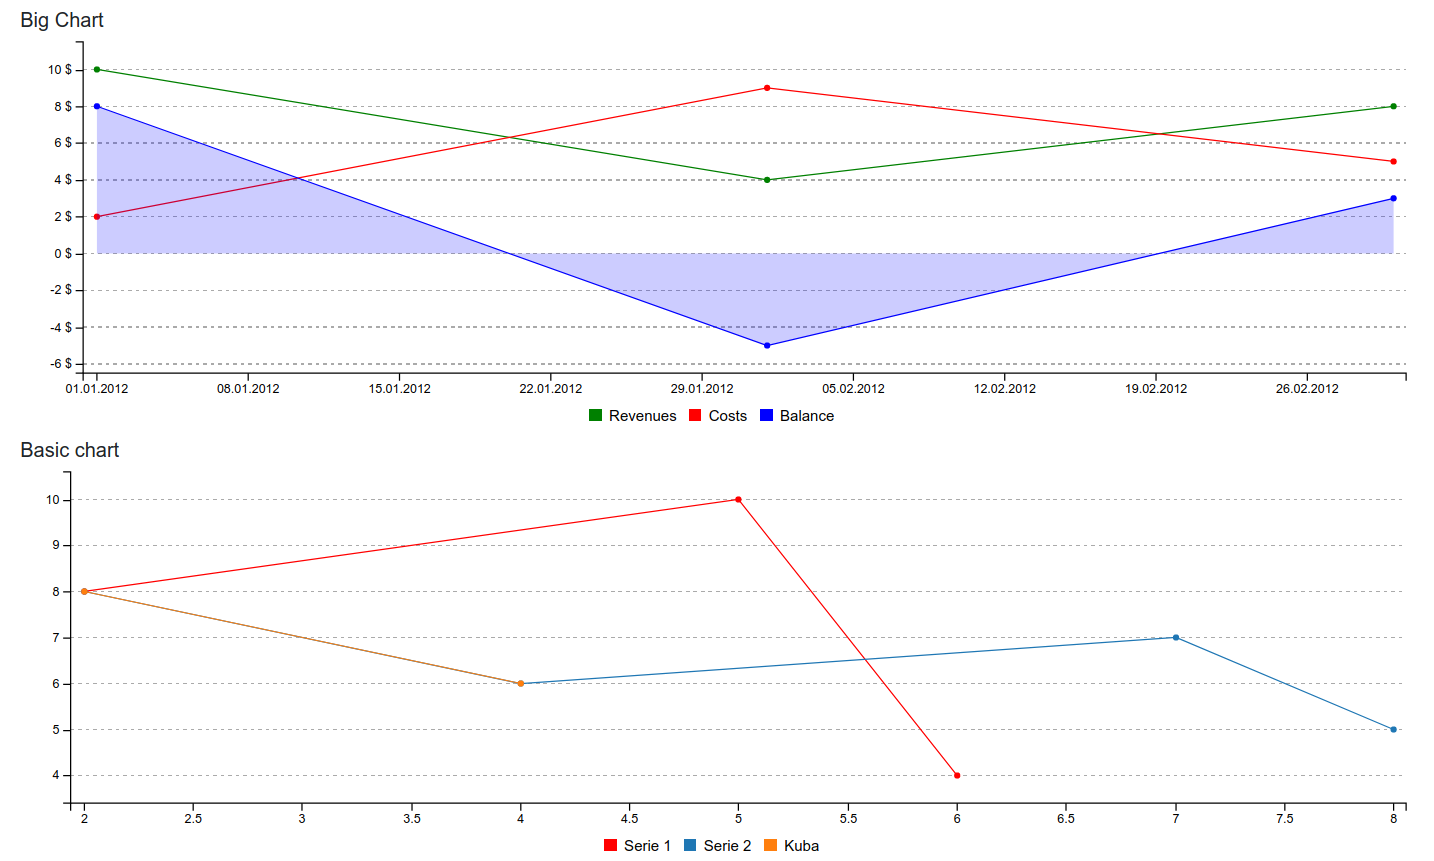
\includegraphics[width=\textwidth]{img/Graf.png}
    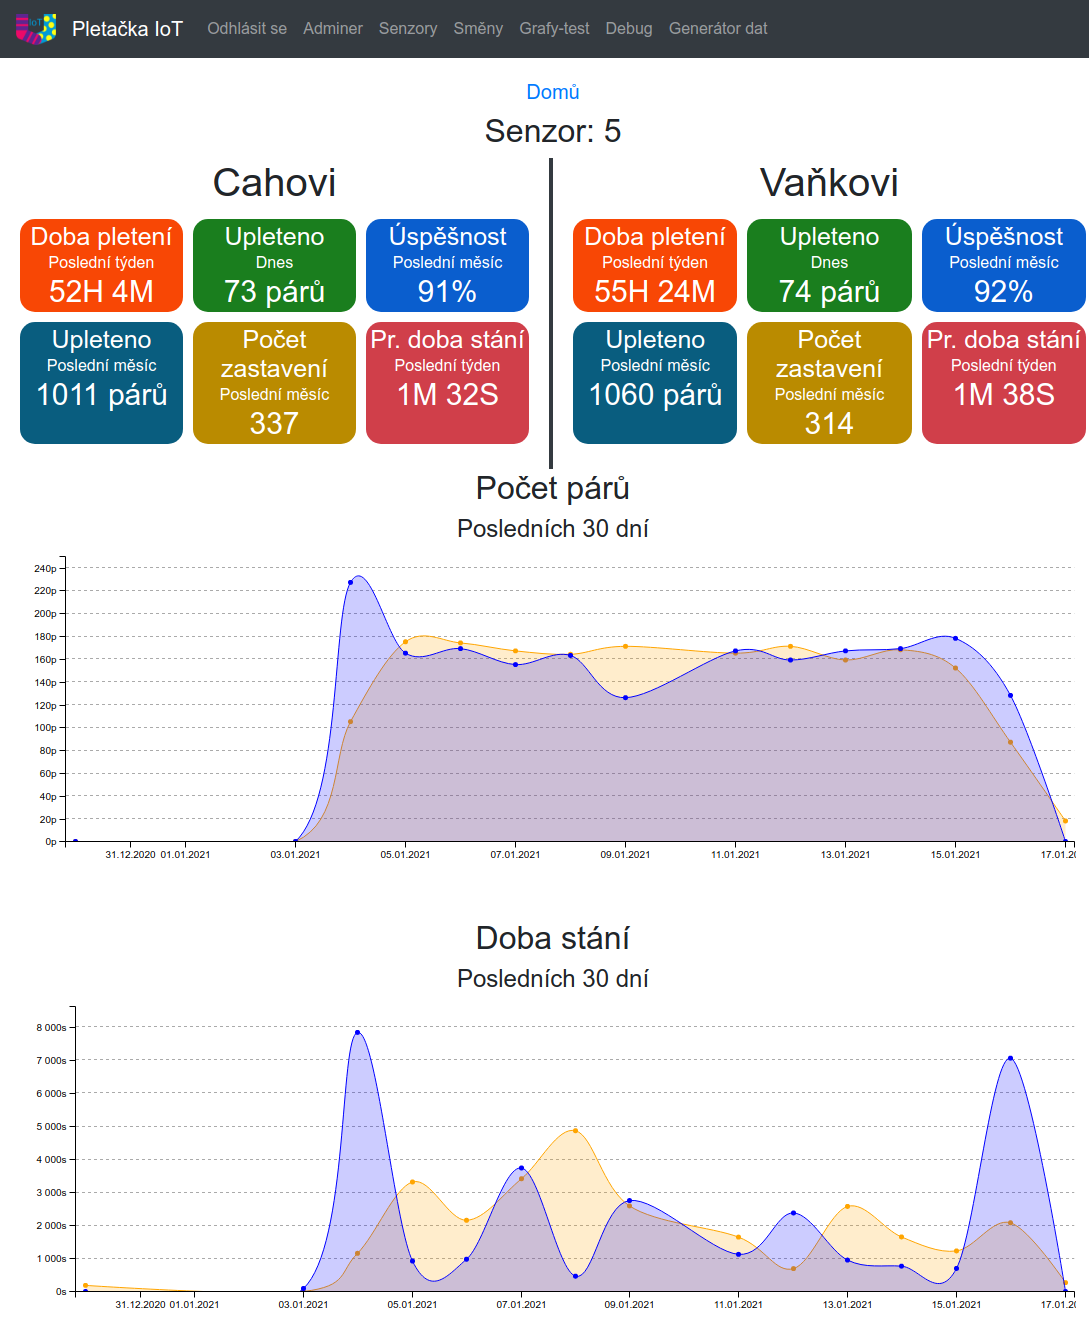
\includegraphics[width=\textwidth]{img/prehled.png}
    \caption{Přehled ze senzoru}
    \label{fig:webSenzory}
\end{figure}


\fxnote[author=JPA]{\textcolor{mygreen}{Aktualizovat grafy/obrázky}}


\subsection{Správa senzorů}
Pro vstup do této sekce je nutné uživatelské přihlášení do systému.
Stránka pak nabízí přehled senzorů s~jednotlivými možnostmi úpravy (viz obrázek \ref{fig:webSpravaSenzoru}).

% První z~odkazů vede na aktuální přehled ze senzoru.
% Druhý řeší editaci senzoru a~poslední maže vybraný senzor.
% \fxnote[author=JPA]{\textcolor{mygreen}{"První z~odkazů vede na aktuální přehled ze senzoru. Druhý řeší editaci senzoru a~poslední maže vybraný senzor." = není to dostatečně jasné}}

\begin{figure}[htbp]
    \centering
    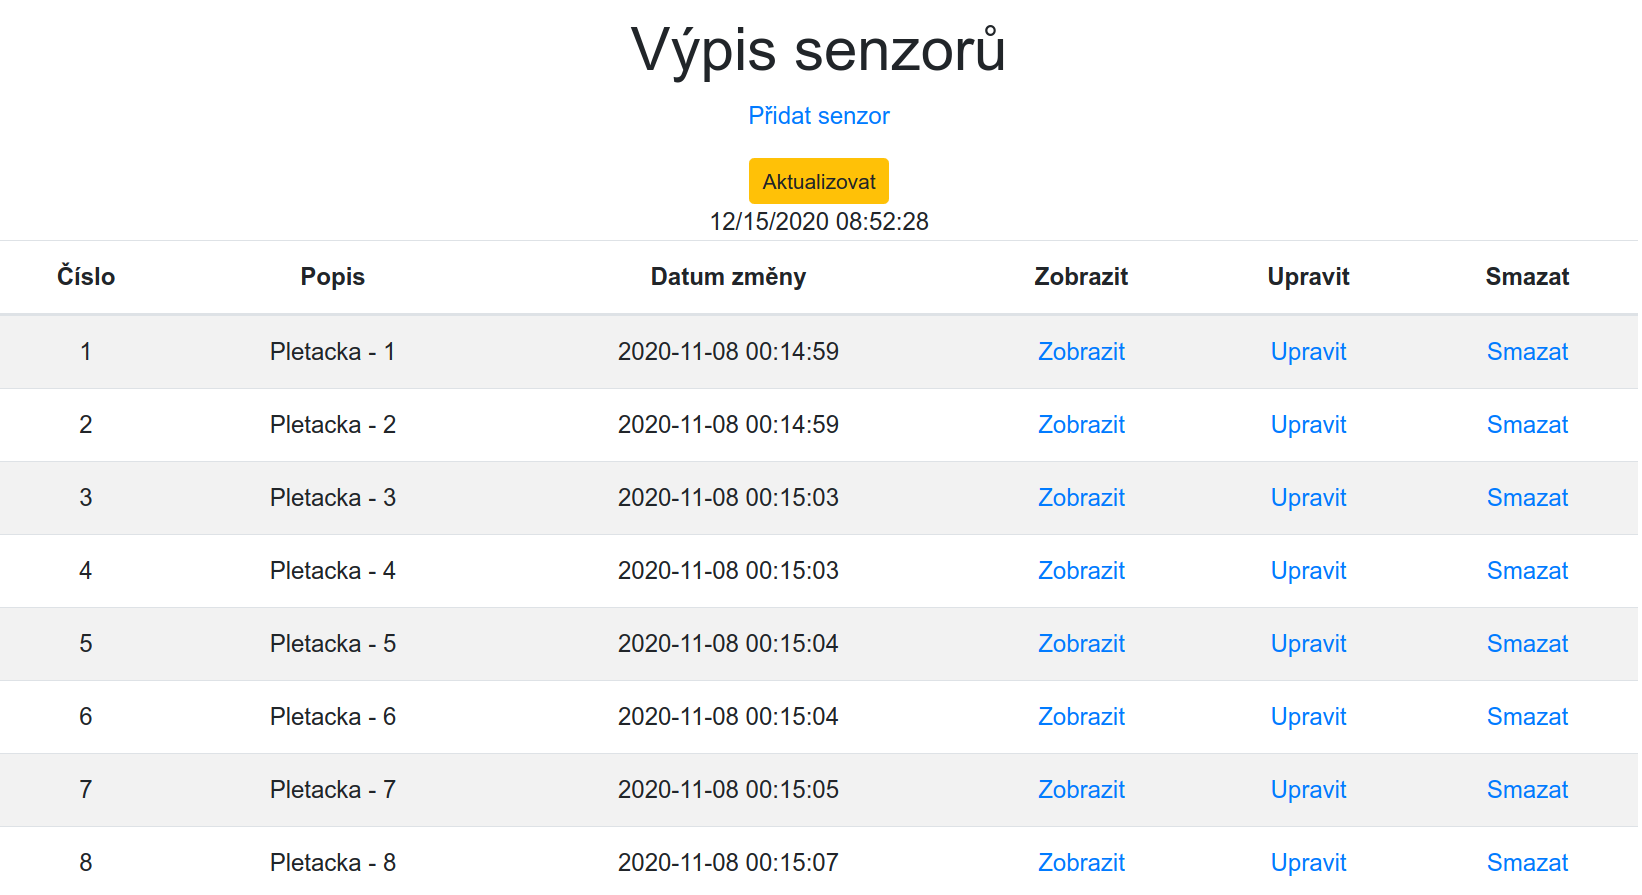
\includegraphics[width=\textwidth]{img/Edit.png}
    \caption{Správa senzorů}
    \label{fig:webSpravaSenzoru}
\end{figure}

\subsection{Nastavení směn}
Jednoduchá stránka na které se nastavuje pořadí směn.
Střídání směn probíhá pravidelně po týdnech, proto je nastavení velmi jednoduché (viz obrázek \ref{fig:webSmeny})

\begin{figure}[htbp]
    \centering
    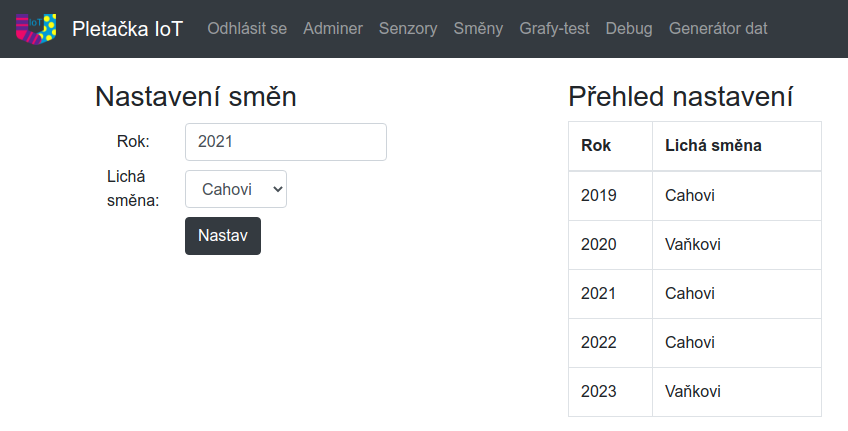
\includegraphics[width=\textwidth]{img/smeny.png}
    \caption{Nastavení směn}
    \label{fig:webSmeny}
\end{figure}

%SECTION
\section{Databáze}
Databáze je rozdělená do dvou skupin tabulek.

První skupina tabulek je nastavovací, jedná se o~hlavní nastavení webu, nastavení směn a~o~tabulku s~uživateli a~jejich oprávněním.

Druhá skupina je senzorová.
Každý senzor zde má pět tabulek na ukládání svých dat.
První senzorová tabulka ukládá čistá nezpracovaná data posílaná přímo ze senzoru.
Zbylé čtyři~tabulky jsou databázové výběry různých časových úseků, jde o~výběr hodinový, denní, měsíční a~roční.  
Tyto tabulky se vytvářejí automaticky pomocí výběrového API. 
Struktura tabulek je vyobrazena ve schématu \ref{fig:databaze}.


\begin{figure}[htbp]
    \centering
    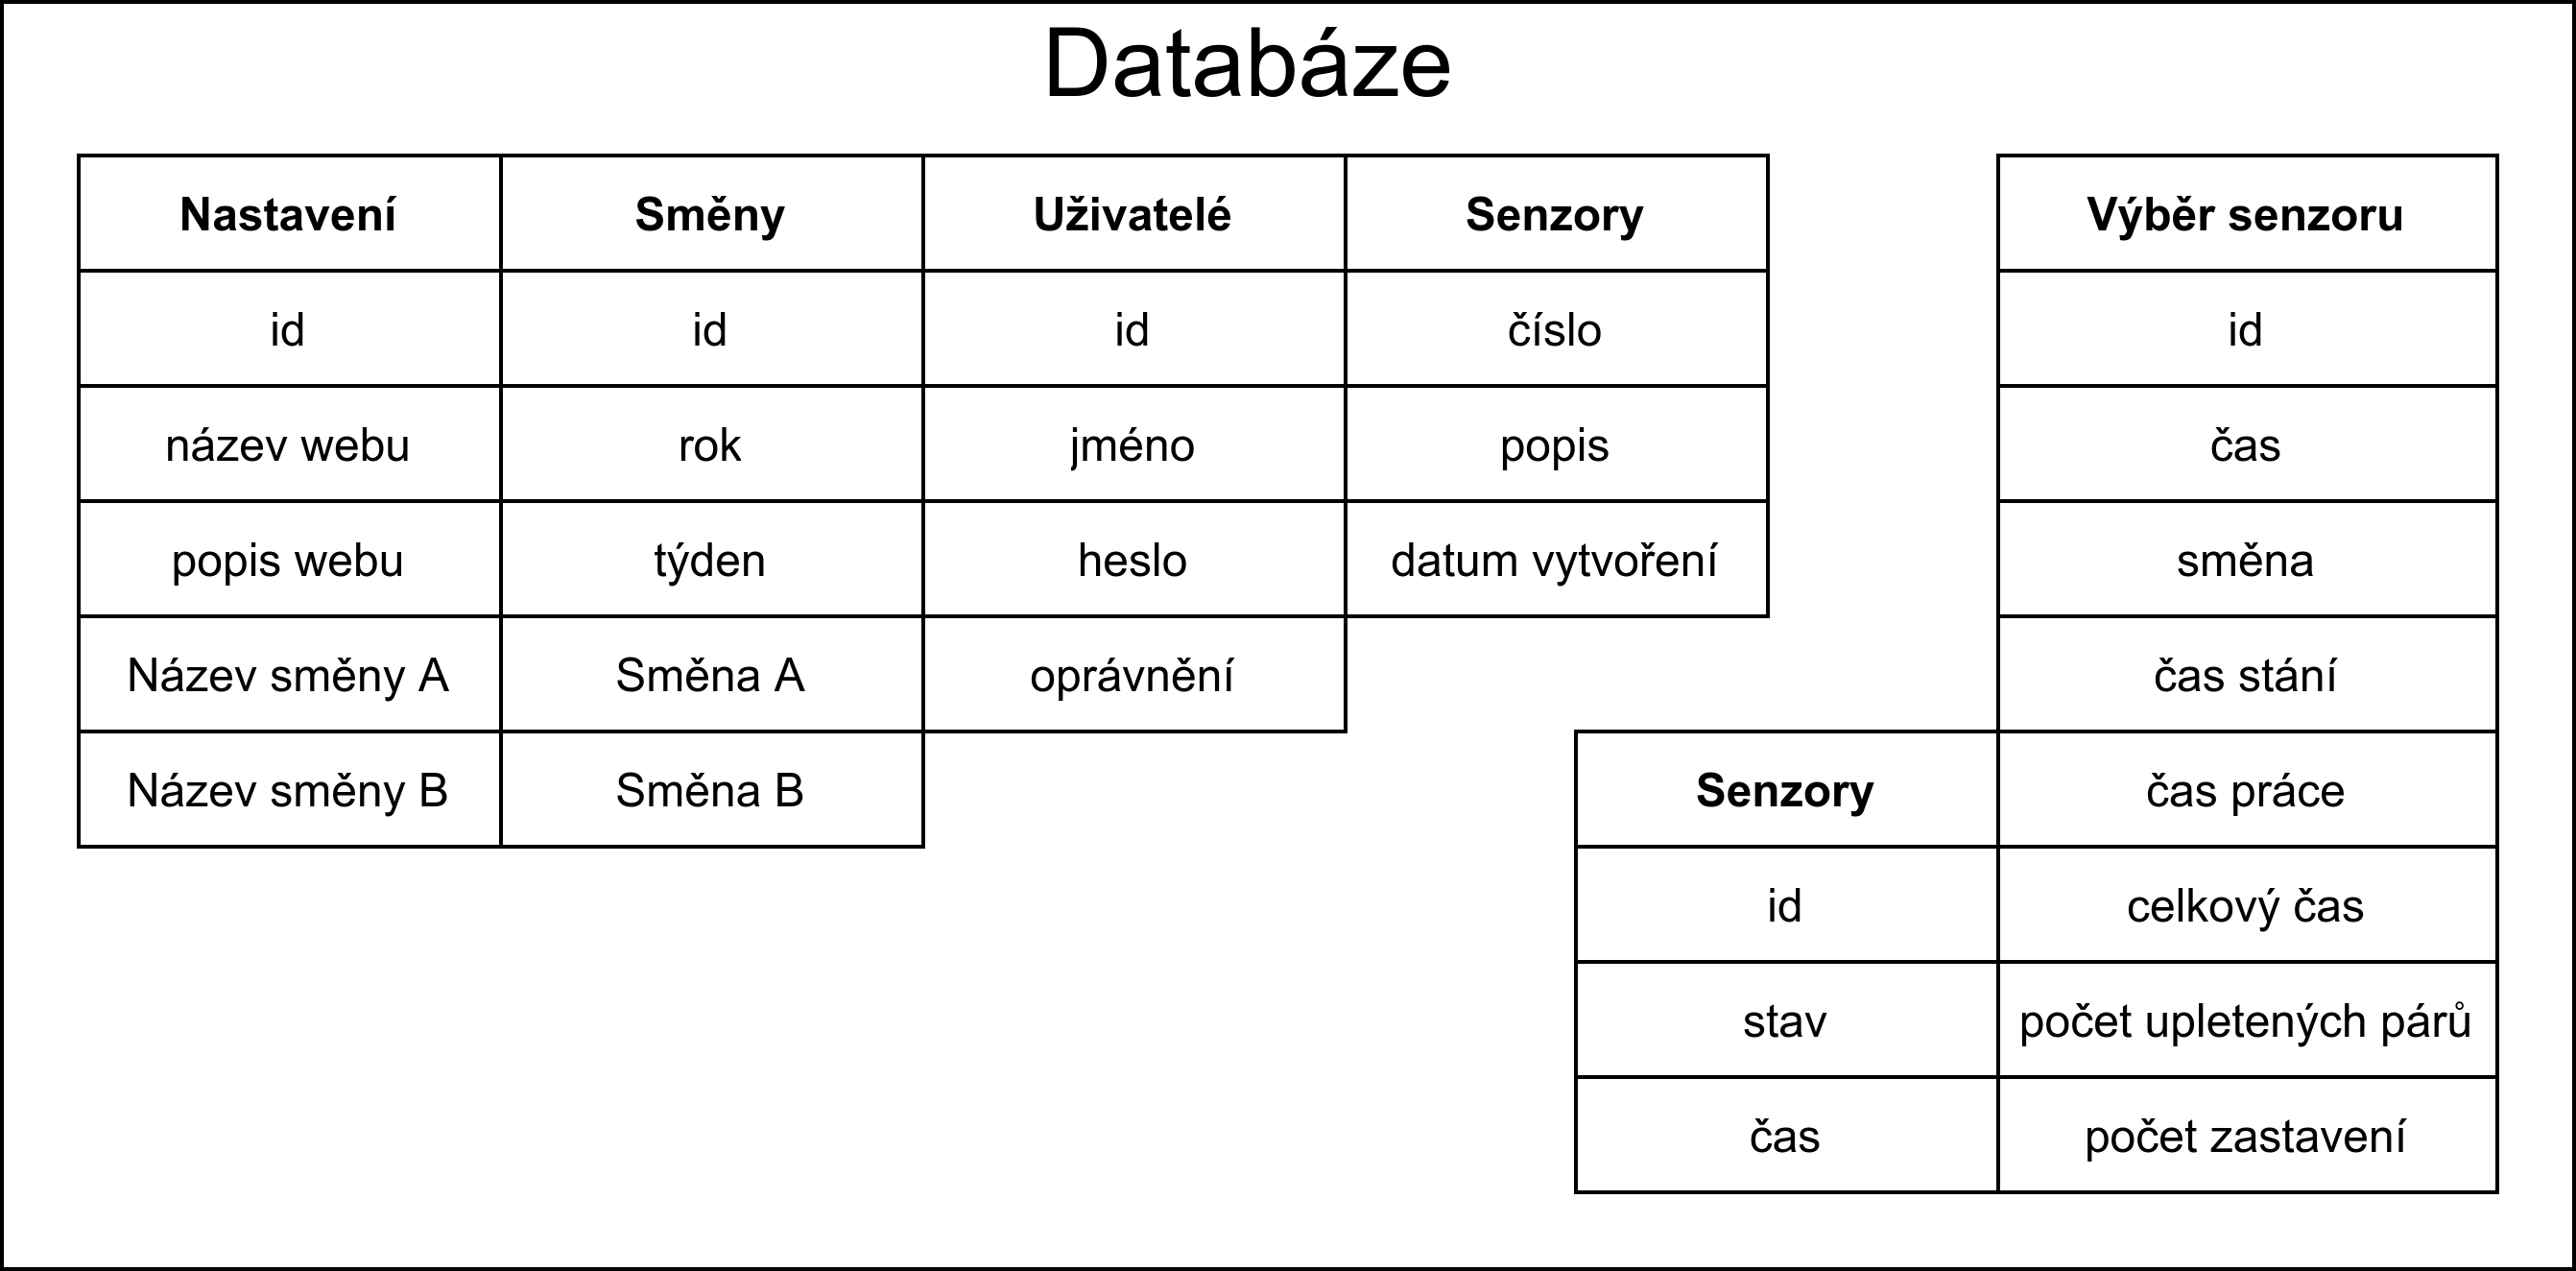
\includegraphics[width=\textwidth]{img/Databaze.png}
    \caption{Struktura databáze}
    \label{fig:databaze}
\end{figure}


\fxnote[author=JPA]{\textcolor{mygreen}{Možná bychom se mohli pobavit o~úpravě "Struktura databáze" obrázku.}}



\section{Funkcionalita}

Systém je schopen


\newpage